\section{Related Work}
\label{sec:related_work}

The scalability model derived in this work is inspired by the symptotic scalability framework outlined in \cite{symptotics_journal}, which has been previously applied to content-agnostic static networks \cite{symptotics_framework_scalability} and mobile networks \cite{scal_analysis_mobility}. {\color{blue}We provide several differences and additional analysis here compared to these works, which mainly stem from our use of QoI requirements instead of static data rates. The first difference is that we are able to evaluate performance and scalability under timeliness constraints, which is not possible under any of these prior works. Second, we illustrate the effects on an application's performance, which is not linear with respect to data rates in most cases. Additionally, we provide a formulation that includes parameters characterized by random variables. This improved modeling allows us to characterize expected delays with a probability distribution, which the previous works do not provide.}

Other works characterize the capacity of wireless networks, like \cite{li_capacity, gupta2000capacity}, but all do so by considering how networks scale asymptotically or by analyzing specific network instances instead of developing a general model. {\color{blue}Experimental techniques, like Response Surface Methodology \cite{khuri2010response}, discrete-event simulators \cite{ns3}, and real wireless network testbeds \cite{iot_lab_exp_platform, wsn_testbed, wisebed} may be applied to solve the problem we do, and, in fact, after finalizing a network design, implementing one of these methods to further verify capabilities is desirable. The anticipated applications of this work, however, are different in that either there is not enough time to develop a realistic simulation or implementation, or the goal is to evaluate a number of combinations of design choices, such that implementing each possible combination and/or running trials over the sets of independent parameters would be too time-intensive.}

A large number of works provide definitions for QoI and frameworks that utilize it.  We will address only the most relevant ones here.  Primarily, QoI has been considered from a number of angles including routing \cite{quality_aware_routing_tan}, scheduling/rate control \cite{toward_qoi_rate_control,explor_vs_exploit}, and impact on usage of network resources \cite{qoi_aware_mobile_apps}. Our focus is on a broader scale here, though, modeling scalability and limitations of an entire network.  

%The work in \cite{qoi_aware_mobile_apps} evaluates the impact of varying QoI requirements on usage of network resources, which is certainly related to this paper.  Our focus is on a broader scale than this work, though, by modeling an entire network instead of a single node as the authors do in \cite{qoi_aware_mobile_apps}.

A framework called Operational Information Content Capacity (OICC) is outlined in \cite{oicc_journal}, which describes the obtainable region of QoI, a notion similar to the \emph{scalably feasible QoI region} developed here. OICC differs, though, in the fact that it does not provide any method for determining the possible size of the network or impact of network design choices like medium access protocols. We also note that a notion similar to QoI satisfiablility was considered in \cite{qoi_outage} which addresses resource allocation for long-term average QoI outage satisfaction. However, the focus of \cite{qoi_outage} is energy-efficient scheduling and power allocation in a single-hop three-node network rather than scalability. 

In Section \ref{sec:qoi_model}, we use similarity-based image collection as an example of an application that is best evaluated using QoI.  This application has previously been considered in \cite{photonet} and \cite{mediascope}. Our scope is greater than that of \cite{photonet}, which does not consider attributes of timeliness, nor the consideration of transmission rates and network topology.  We use the same similiary-based image selection algorithm as in \cite{mediascope}, but provide new methods of quantifying QoI.% considers a smartphone application where different queries called Top-K, Spanner, and K-means Clustering are defined.  We use these same similarity-based image selection algorithms, but we provide new methods of quantifying QoI from them.

\begin{figure*}[t!]
\centering
    \subfigure[Top-K: Sum Similarity]{
        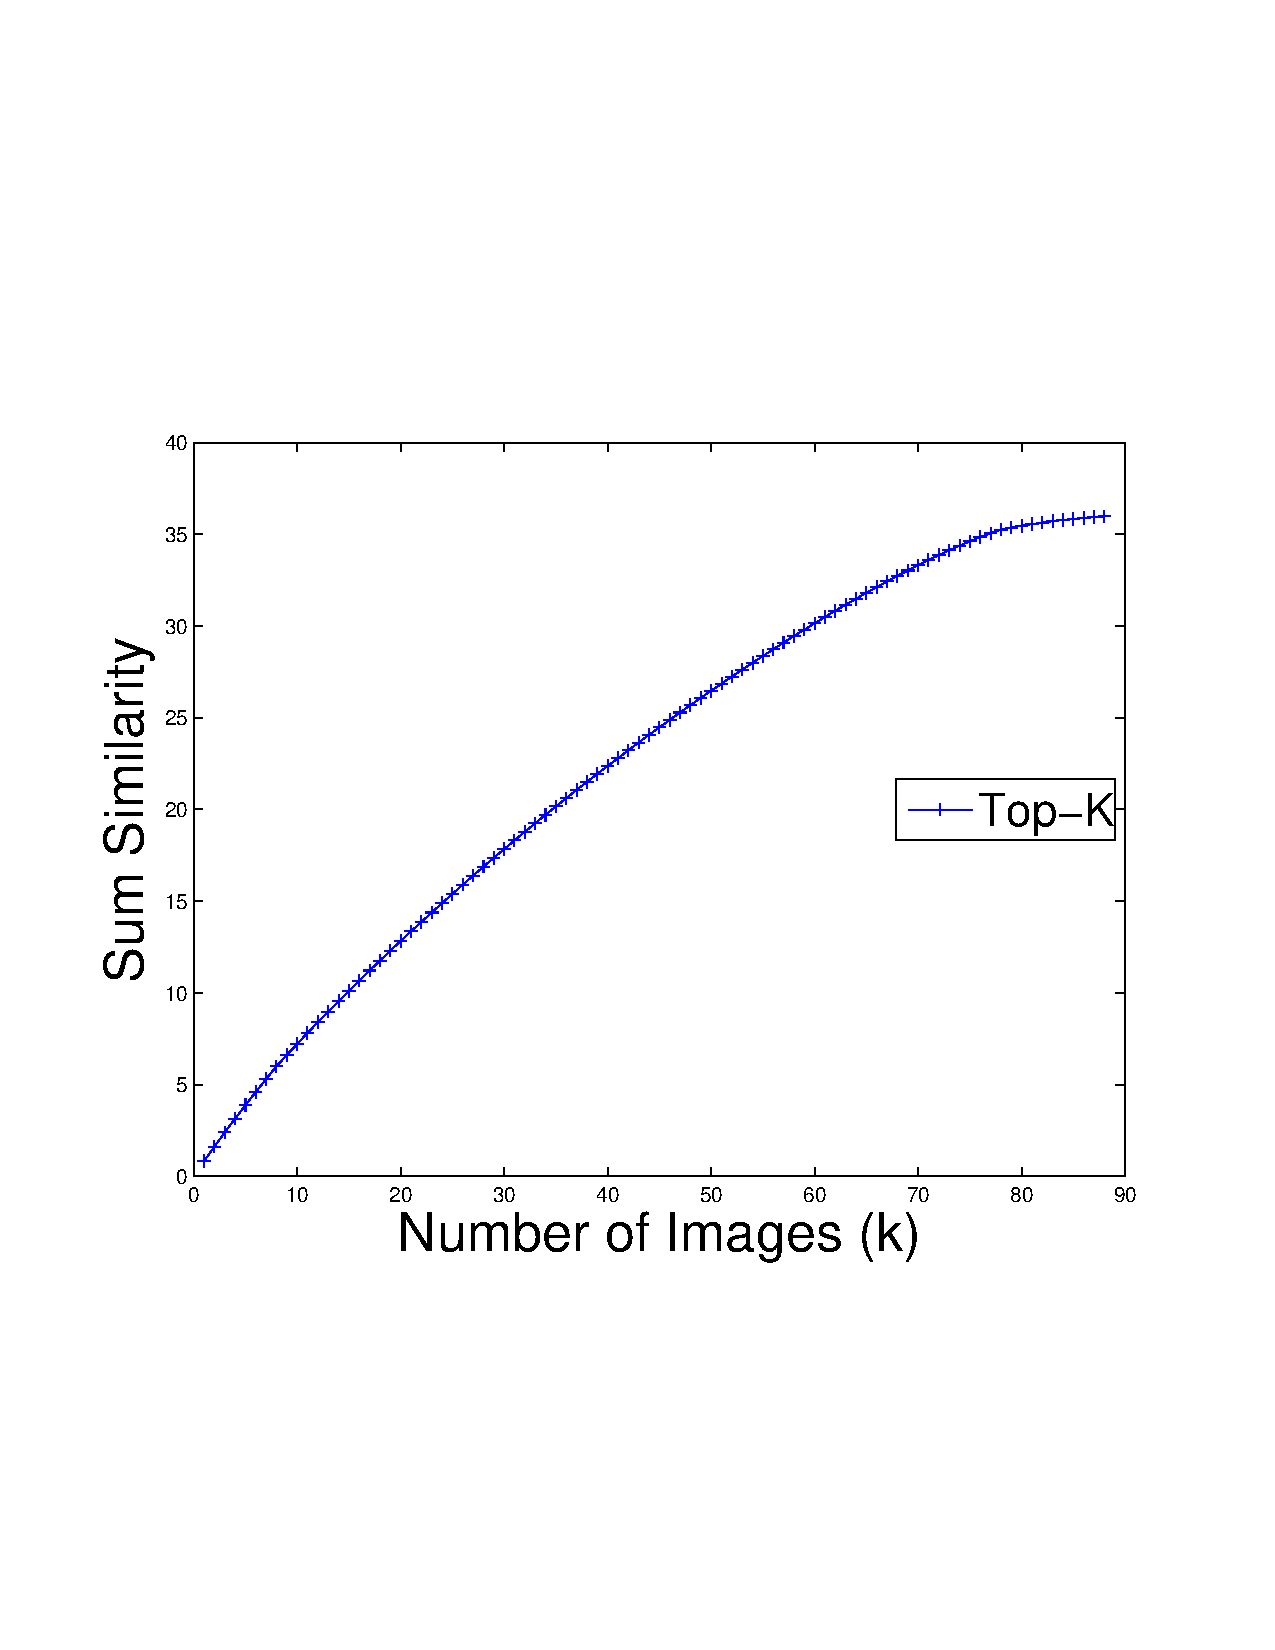
\includegraphics[clip=true, trim = 17mm 65mm 25mm 70mm, scale=0.23]{figures/topk/topk_sum_sim_color.pdf}
        \label{fig:topkSumSim}
        }
    \subfigure[Top-K: Avg. Match Target]{
        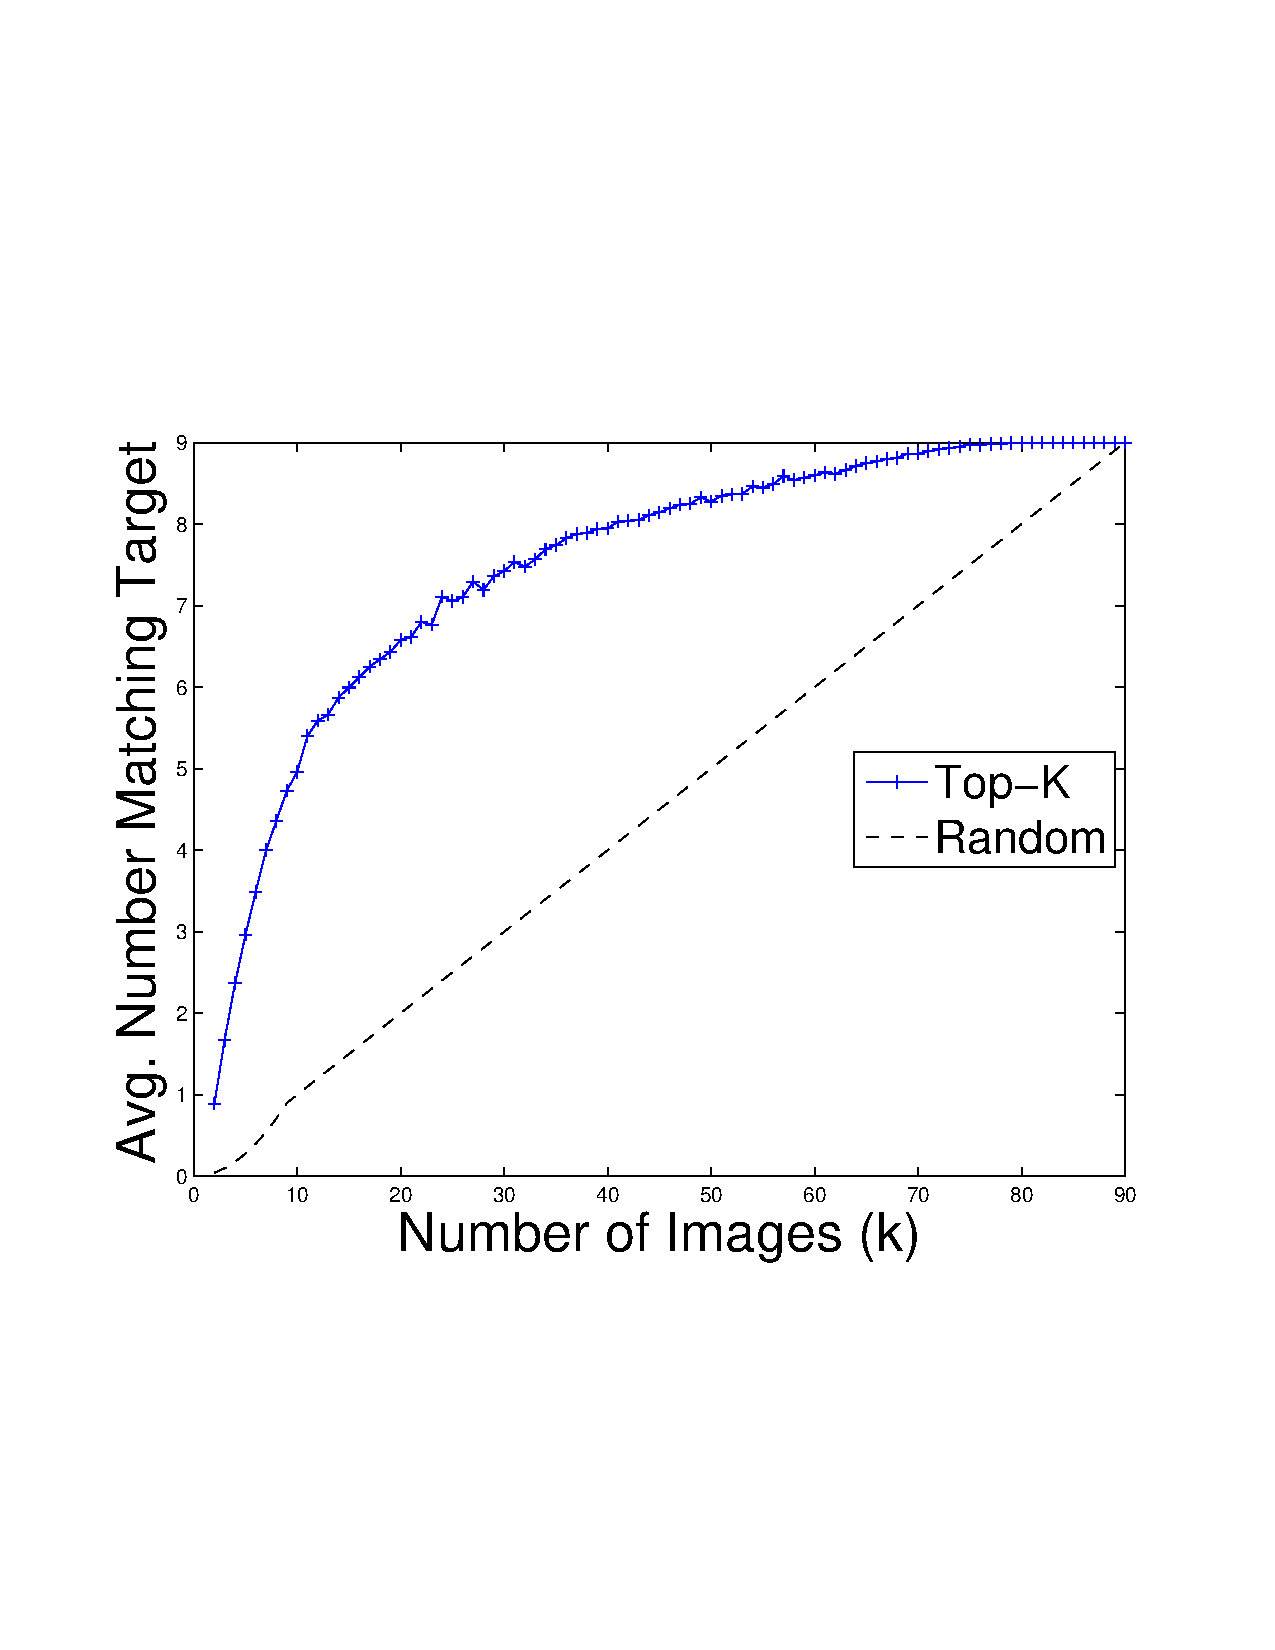
\includegraphics[clip=true, trim = 17mm 65mm 25mm 70mm, scale=0.23]{figures/topk/avg_num_matching_color.pdf}
        \label{fig:topkAvgNumSameSet}
        }
    \subfigure[Spanner: Sum Dissimilarity]{
        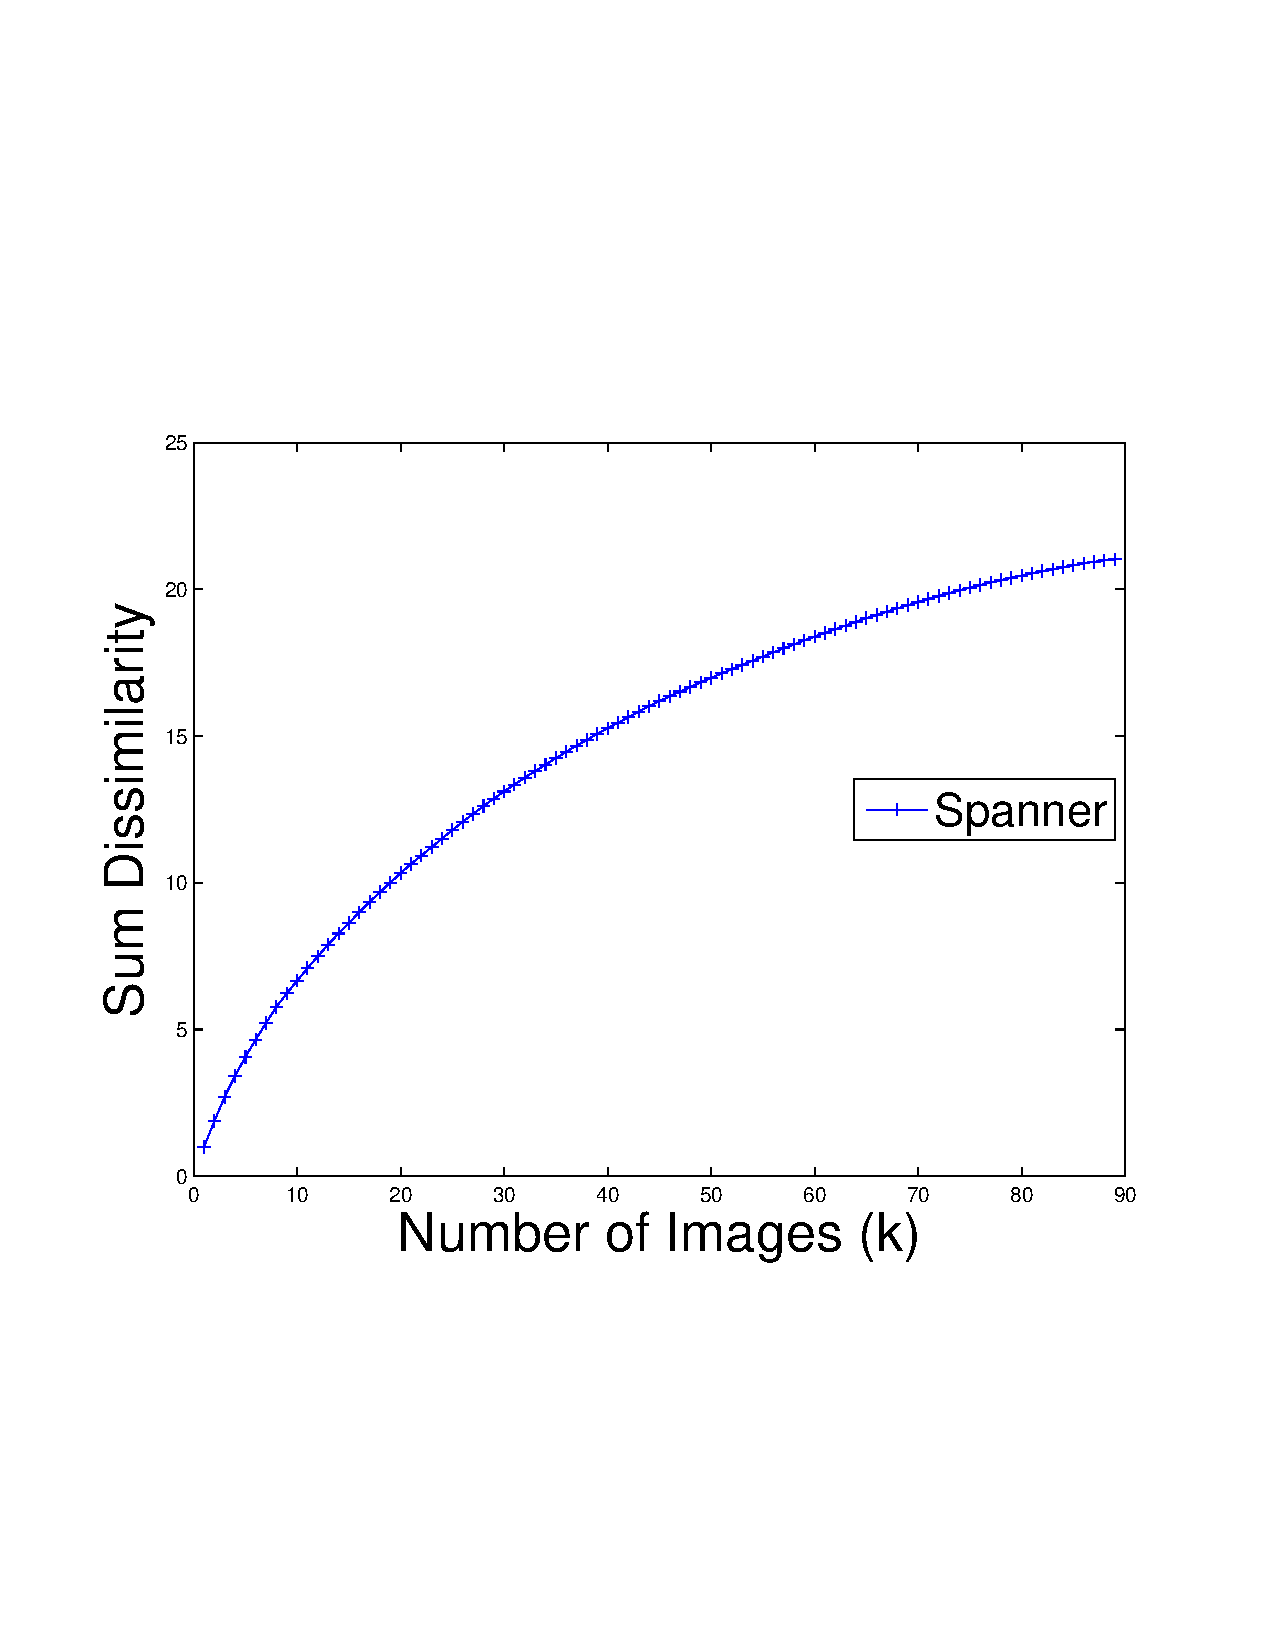
\includegraphics[clip=true, trim = 17mm 65mm 25mm 70mm, scale=0.23]{figures/spanner/spannerCumulativeDist_color.pdf}
        \label{fig:spanSumDissim}
        }
    \subfigure[Clustering: Cover All Sets]{
        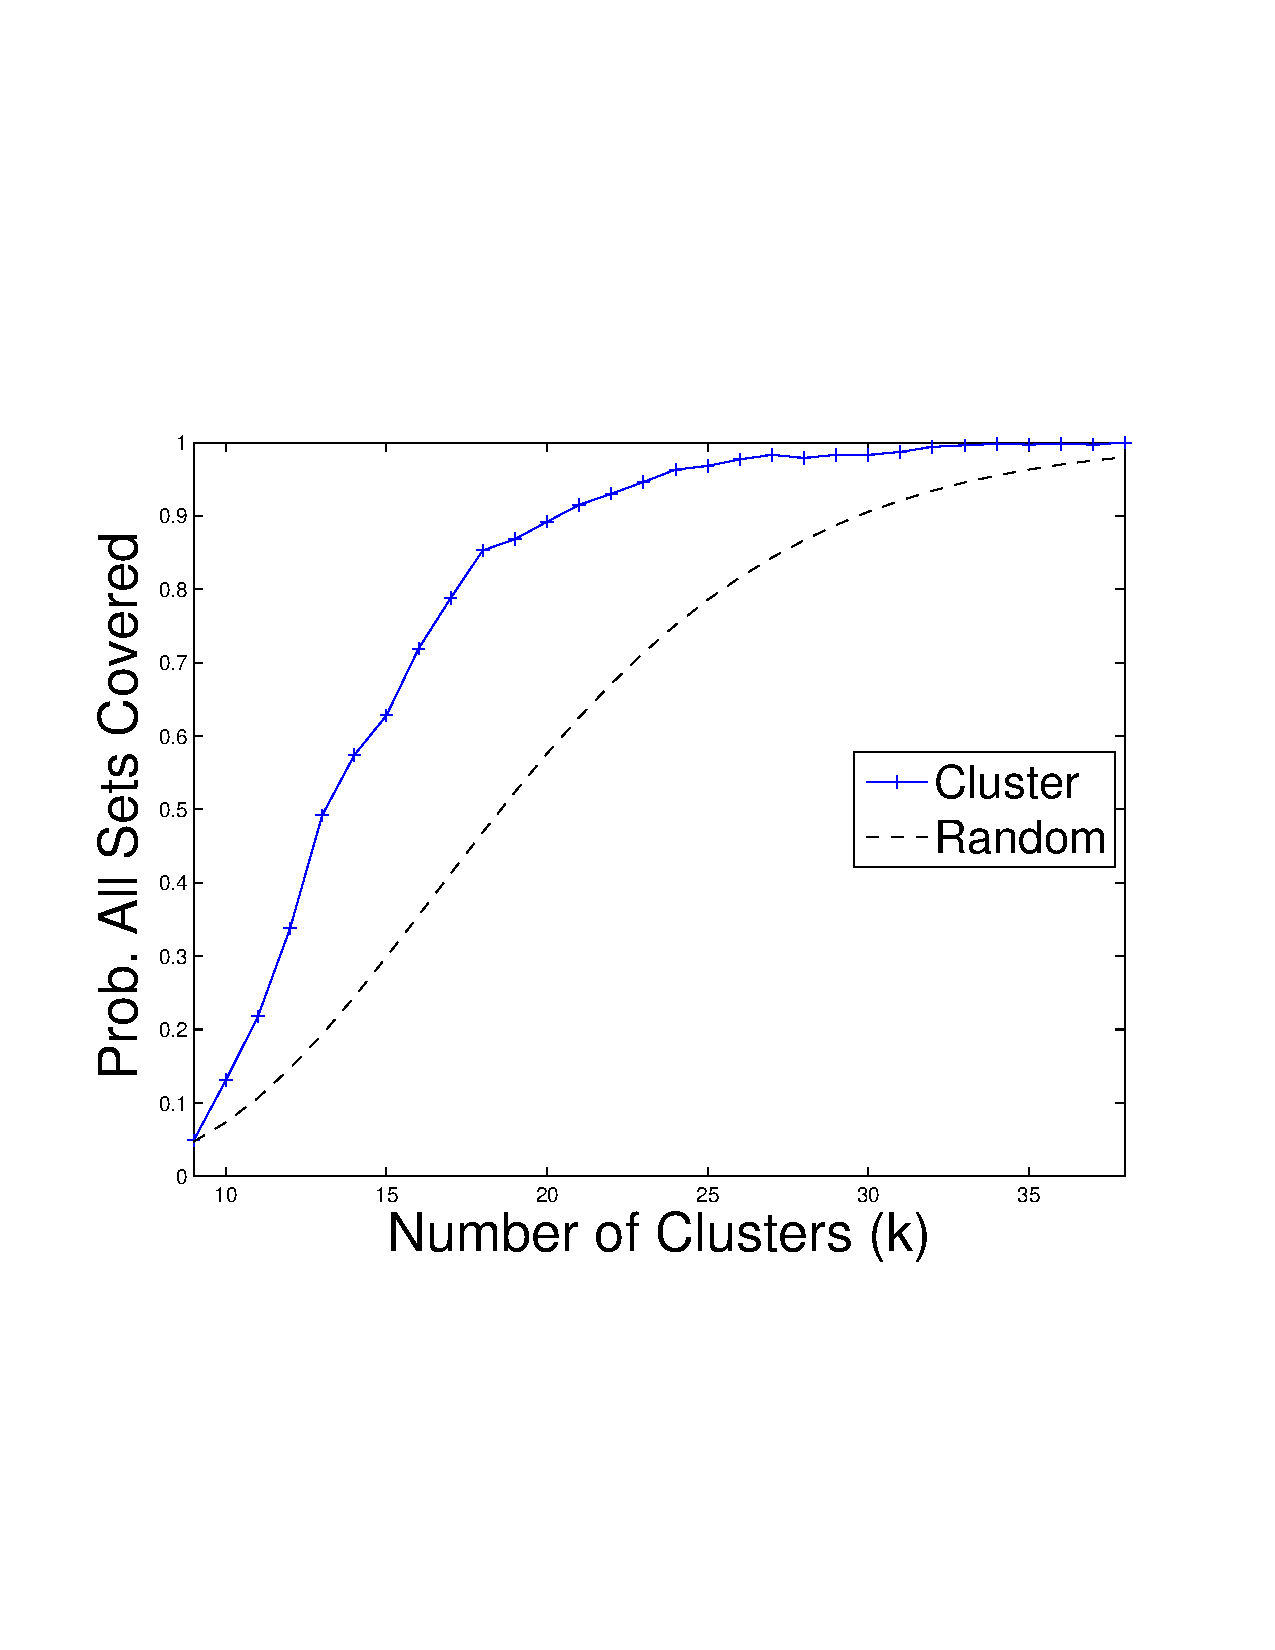
\includegraphics[clip=true, trim = 16mm 65mm 25mm 70mm, scale=0.23]{figures/cluster/perc_all_sets_covered_vary_k_color.pdf}
        \label{fig:clusterAvgNumSetsCov}
        }        
   \caption{Completeness metrics for the three image selection algorithms. Each exhibits a diminishing return as more images are added.}
   \label{fig:completeness_exp_results}
   \vspace{-4mm}
\end{figure*}